\section{Background and Related Benchmarks}
\label{sec:background}

This appendix situates \textbf{m2sv} among recent benchmarks for spatial
reasoning and cross-view understanding. We focus on the benchmarks most adjacent
to \textbf{m2sv} and clarify how our task differs from them.

\subsection{What Spatial Capability Does m2sv Measure?}
\label{sec:background-capability}

\textbf{m2sv} isolates a single spatial reasoning primitive:
\emph{inferring camera heading by aligning an egocentric street-level view with a
north-up overhead map at a known location}. Each example fixes the geographic
position and varies only the candidate viewing direction, converting orientation
from a nuisance variable into the primary reasoning target. This formulation
removes global localization and retrieval from the task, forcing explicit
reasoning about road topology, landmark placement, and allocentric--egocentric
transformations under real-world ambiguity.

\subsection{Closest Related Benchmarks}
\label{sec:background-closest}

\paragraph{CityCube.}
CityCube \citep{citycube2026} benchmarks cross-view spatial reasoning in urban environments
and reports recurring failures such as directional confusion and viewpoint
inconsistency.
Compared to CityCube's broader suite of tasks, \textbf{m2sv} intentionally
constrains the problem to a \emph{single-step heading decision at a fixed
location}, enabling controlled measurement of how structural ambiguity (e.g.,
symmetry) affects orientation inference.

\paragraph{UrBench.}
UrBench \citep{urbench2024} is a multi-view urban benchmark covering diverse task types
(including tasks related to localization and orientation in urban scenes).
While UrBench contains cross-view components that are conceptually adjacent to
\textbf{m2sv}, its scope spans multiple urban reasoning dimensions.
In contrast, \textbf{m2sv} focuses narrowly on \emph{heading inference} by
aligning an overhead map with a Street View observation at a known intersection,
thereby isolating allocentric--egocentric alignment as the primary bottleneck.

\paragraph{MindCube.}
MindCube \citep{yin2025spatialmental} evaluates whether VLMs can maintain coherent spatial mental
models from limited observations, including perspective-taking and consistency
under viewpoint changes. It motivates ``map-then-reason'' style approaches that
explicitly produce intermediate spatial representations before answering.
Although m2sv shares the theme of viewpoint-consistent spatial reasoning,
\textbf{m2sv} differs in its \emph{real-world cross-view} setting (overhead map
$\leftrightarrow$ street-level imagery) and its emphasis on resolving ambiguous cross-view alignment by escalating
from coarse, unreliable cues to finer-grained spatial evidence at a concrete
intersection.

\paragraph{Ego3D-Bench.}
Ego3D-Bench \citep{ego3dbench2025} evaluates outdoor spatial reasoning using ego-centric,
multi-view observations and shows a substantial human--model gap. The associated
Ego3D-VLM framework improves performance by introducing an explicit
cognitive-map style intermediate representation derived from estimated 3D
coordinates. These results support the broader hypothesis that structured
intermediate spatial state can benefit VLM reasoning; however, whether similar
representations help \textbf{m2sv} depends on how well they align to the
map--street-view transformation and the uncertainty/ambiguity present in real
Street View observations.

\subsection{Relation to Cross-View Geo-Localization (CVGL)}
\label{sec:background-cvgl}

Cross-view geo-localization (CVGL) studies the correspondence between ground-level imagery
(e.g., street-view panoramas or limited-FoV views) and overhead imagery (e.g., satellite/aerial),
with the dominant formulation cast as \emph{retrieval}: a ground query is matched against a
geo-tagged overhead database and evaluated using retrieval metrics such as Recall@K
(e.g., on CVUSA/CVACT-style benchmarks and follow-ups)~\cite{workman2015cvusa,liu2019lending,zhu2021vigor,huang2024cvcities}.
While some benchmarks extend viewpoints~\cite{zheng2020university1652},
the core objective in these settings remains location retrieval rather than isolating directional reasoning.

Because cross-view appearance and geometry differ substantially, many CVGL methods incorporate
mechanisms to account for unknown \emph{orientation/alignment} between ground and overhead views.
Representative approaches include explicitly encoding orientation cues~\cite{liu2019lending},
using polar transforms and correlation-style matching to estimate azimuth alignment during localization~\cite{shi2020wherelooking},
or estimating cross-view alignment/orientation as part of the matching pipeline~\cite{zhu2021revisiting}.
Recent work also explores graph-structured urban priors and bearing-aware filtering on top of retrieval~\cite{shore2025spagbol},
and orientation-free formulations for cross-view matching have been proposed~\cite{hu2025oriloc}.
However, even when orientation is modeled or estimated, it is typically \emph{in service of improving retrieval},
i.e., heading is not the primary target variable.

\textbf{m2sv} complements CVGL by \emph{fixing the location} and asking the model to infer
\emph{orientation directly}. This inversion removes global retrieval shortcuts (e.g., relying on distinctive
place identity in a large gallery) and makes directional reasoning the dominant challenge.

\subsection{Structural Difficulty and Symmetry}
\label{sec:prior-difficulty}

Unlike many recent vision--language benchmarks, which define difficulty primarily
through semantic complexity or multi-step reasoning, spatial reasoning difficulty
has a long history of being operationalized through geometric transformation.
In cognitive psychology, difficulty is closely linked to mental effort and response
time (RT): classic results show that RT increases linearly with the angular
displacement required to align two objects, suggesting a process akin to physical
mental rotation~\citep{shepard1971mental}.
By contrast, contemporary VLM benchmarks often categorize difficulty by reasoning
depth or semantic richness (e.g., number of symbols, hops, or compositional steps),
as in MathVista~\citep{lu2024mathvista} or MapQA~\citep{li2025mapqa}, potentially
underrepresenting the role of intrinsic geometric ambiguity.

\textbf{m2sv} introduces \emph{structural difficulty} rooted in intersection
geometry and symmetry. Symmetric or near-symmetric intersections induce multiple
plausible orientations at a coarse level, creating ``symmetry traps'' that cannot
be resolved by semantic pattern matching alone.
Breaking these traps requires escalation to finer-grained spatial cues
(e.g., lane markings, curb geometry, subtle landmark placement), a process that
mirrors increased human RT in geometric alignment tasks.
This framing connects classic findings on mental rotation
to modern observations of allocentric--egocentric failures in VLMs,
and isolates a form of difficulty that is intrinsic to the scene structure itself.




\begin{table}[t]
  \centering
  \caption{Summary statistics of the m2sv-20k dataset.}
  \label{tab:dataset-stats}
  \begin{tabular}{l r}
    \toprule
    Statistic & Value \\
    \midrule
    Number of examples & 20,000 \\
    Number of cities & 32 \\
    Candidate directions (median) & 3 \\
    Street View distance (median) & 2.05 m \\
    Street View distance (95\%) & 4.51 m \\
    \bottomrule
  \end{tabular}
\end{table}

\begin{table}[t]
  \centering
  \caption{Cross-benchmark evaluation for Qwen3-VL-8B variants.}
  \label{tab:transfer}
  \begin{tabular}{l c c c c c}
    \toprule
    Model & MMMU & MME-Cog/Per & MMStar & Omni3D \\
    \midrule
    Base & 0.556 & 643 / 1721 & 0.604 & 0.388 \\
    SFT & 0.574 & 501 / 1525 & 0.574 & 0.372 \\
    SFT+RL & 0.563 & 550 / 1670 & 0.644 & -- \\
    \bottomrule
  \end{tabular}
\end{table}


\begin{table}[t]
  \centering
  \caption{MindCube evaluation suite with varying input/output formats.}
  \label{tab:m2sv-generalization}
  \begin{tabular}{l l c c c}
    \toprule
    Input & Output Format & Base & SFT & SFT+RL \\
    \midrule
    Raw + q & Aug + rsn $\rightarrow$ ans & 34.5 & 34.0 & 33.2 \\
    Aug. + QA & Direct answer & 24.6 & 37.6 & 41.0 \\
    Aug. + QA & Rsn $\rightarrow$ answer & 46.9 & 40.3 & 46.1 \\
    Raw + q & Rsn $\rightarrow$ answer & 38.5 & 36.8 & 36.6 \\
    Raw + q & Map + rsn $\rightarrow$ ans & 34.7 & 33.5 & 35.2 \\
    Raw + q & Direct answer & 27.0 & 34.9 & 34.7 \\
    \bottomrule
  \end{tabular}
\end{table}


\begin{figure*}[t]
  \centering
  \renewcommand{\arraystretch}{1.15}
  
  % ================= Row (a) =================
  \begin{minipage}[t]{\linewidth}
    \centering
    \begin{minipage}[t]{0.24\linewidth}
      \centering
      \vspace{0pt}
      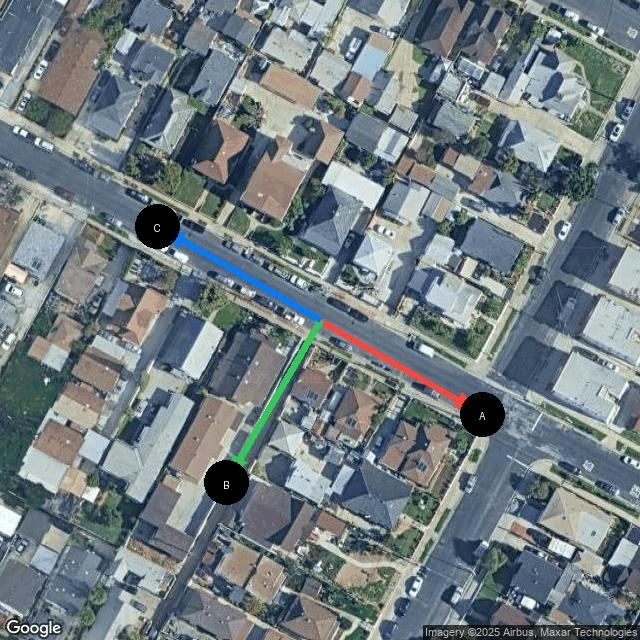
\includegraphics[width=\linewidth]{figures/failure-mode-6-map.jpg}
    \end{minipage}
    \hfill
    \begin{minipage}[t]{0.24\linewidth}
      \centering
      \vspace{0pt}
      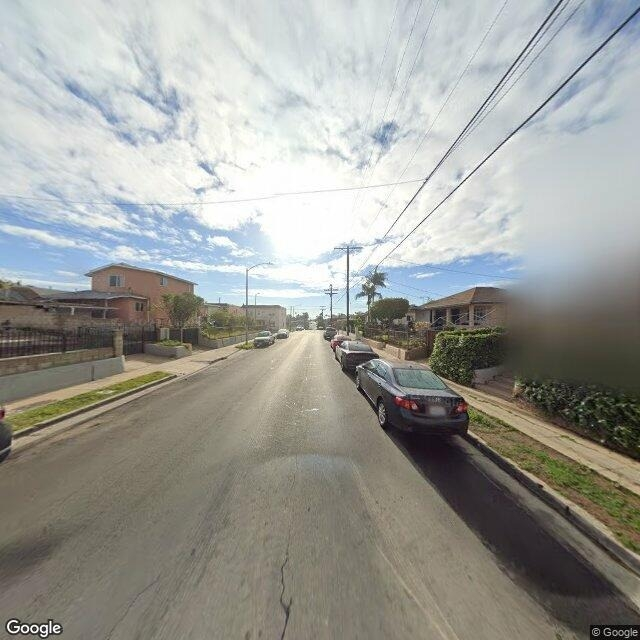
\includegraphics[width=\linewidth]{figures/failure-mode-6-sv.jpg}
    \end{minipage}
    \hfill
    \begin{minipage}[t]{0.50\linewidth}
      \vspace{0pt}
      \fbox{
        \begin{minipage}[t]{\linewidth}
        \footnotesize
        \textbf{Ground truth:} A, \textbf{Prediction:} C
        \medskip

        \textbf{Model trace (excerpt):}
  
        Direction A: This arrow points east-southeast down a relatively narrow residential street. It has no crosswalks visible across its width. \\
        Direction C: This arrow points west-northwest down a much wider road than A and B. This main road clearly has multiple lanes separated by what appear to be painted lines, indicating it's a major thoroughfare. Crosswalks are visible crossing this road.
  
        \medskip
        \textbf{Failure:}
        A and C are two sides of the same street so the road width is the same, but the answer emphasizes the road width as the key factor
        \end{minipage}
      }
    \end{minipage}
  
    \vspace{0.4em}
    \centering
    {\small\textbf{(a) Failure to maintain a consistent spatial representation}}
  \end{minipage}

  \vspace{0.8em}

  % ================= Row (b) =================
  \begin{minipage}[t]{\linewidth}
    \centering
    \begin{minipage}[t]{0.24\linewidth}
      \centering
      \vspace{0pt}
      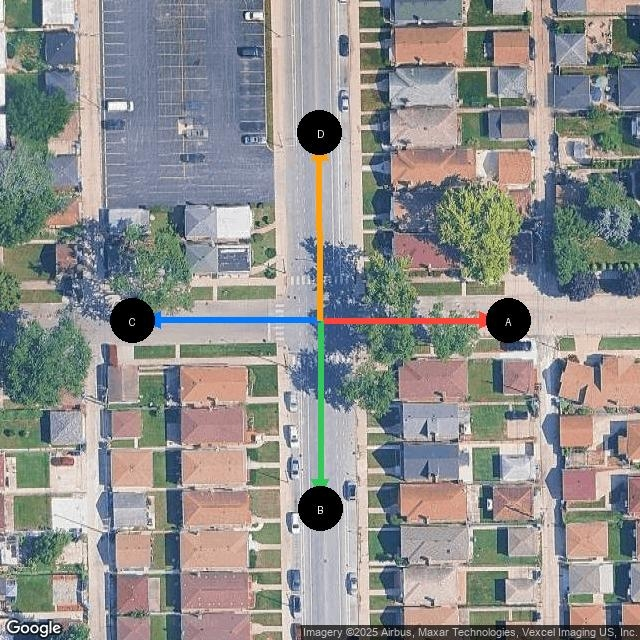
\includegraphics[width=\linewidth]{figures/failure-mode-4-map.jpg}
    \end{minipage}
    \hfill
    \begin{minipage}[t]{0.24\linewidth}
      \centering
      \vspace{0pt}
      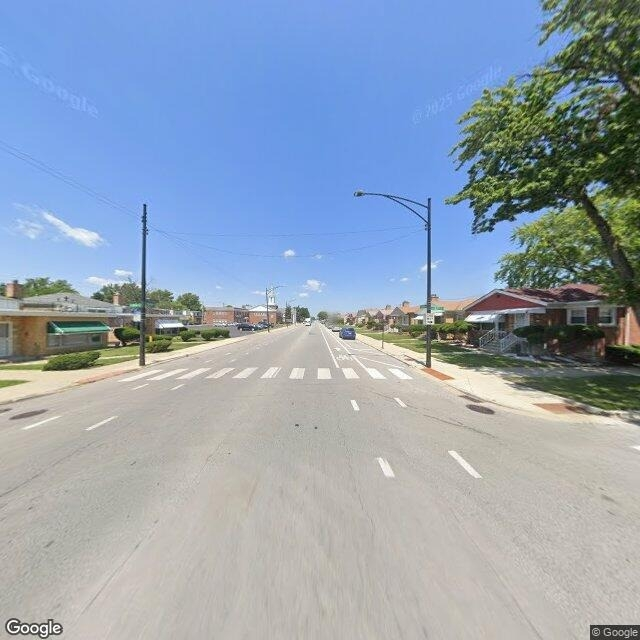
\includegraphics[width=\linewidth]{figures/failure-mode-4-sv.jpg}
    \end{minipage}
    \hfill
    \begin{minipage}[t]{0.50\linewidth}
      \vspace{0pt}
      \fbox{
        \begin{minipage}[t]{\linewidth}
        \footnotesize
        \textbf{Ground truth:} D, \textbf{Prediction:} C
        \medskip

        \textbf{Model trace (excerpt):}
  
        Option D: This view looks up the main, wide road. On the northeast corner (on the right), there is a residential house. On the northwest corner (on the left), there is the commercial building. This arrangement is the opposite of what is seen in the street view photo, where the commercial building is on the left and the house is on the right.
  
        \medskip
        \textbf{Failure:}
        The model correctly identifies left–right relationships but subsequently contradicts its own assignments, losing track of spatial state during verbalization.
        \end{minipage}
      }
    \end{minipage}
  
    \vspace{0.4em}
    \centering
    {\small\textbf{(b) Internal contradiction and state inconsistency}}
  \end{minipage}

  \vspace{0.8em}

  % ================= Row (c) =================
  \begin{minipage}[t]{\linewidth}
    \centering
    \begin{minipage}[t]{0.24\linewidth}
      \centering
      \vspace{0pt}
      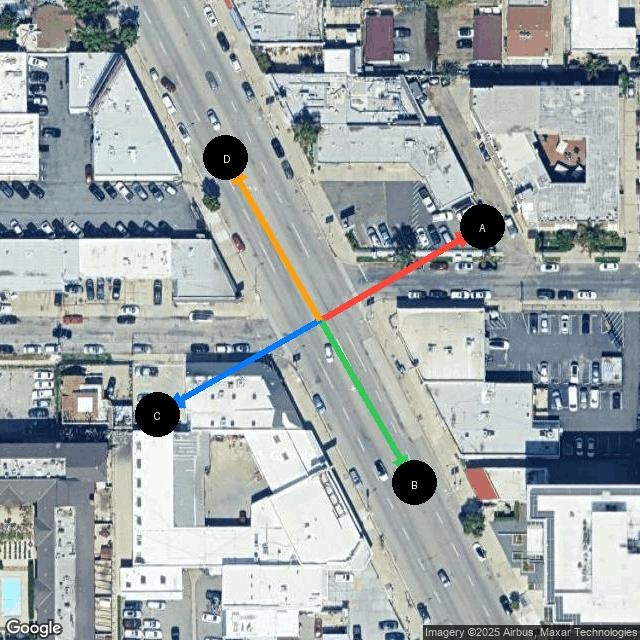
\includegraphics[width=\linewidth]{figures/failure-mode-2-map.jpg}
    \end{minipage}
    \hfill
    \begin{minipage}[t]{0.24\linewidth}
      \centering
      \vspace{0pt}
      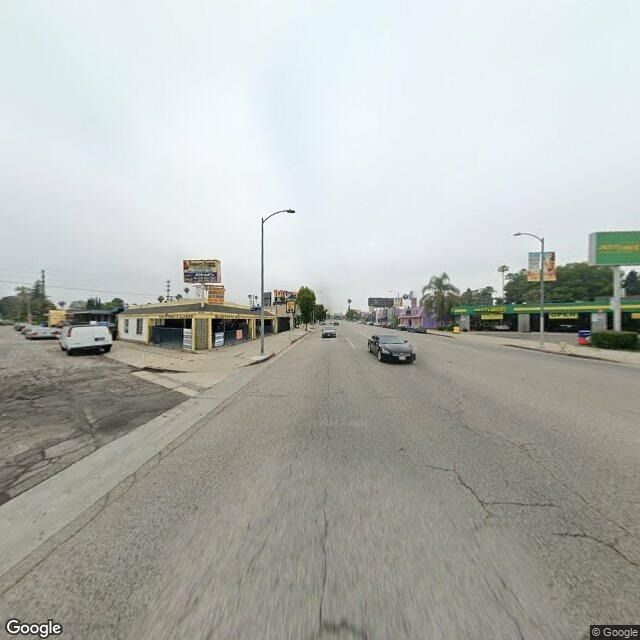
\includegraphics[width=\linewidth]{figures/failure-mode-2-sv.jpg}
    \end{minipage}
    \hfill
    \begin{minipage}[t]{0.50\linewidth}
      \vspace{0pt}
      \fbox{
        \begin{minipage}[t]{\linewidth}
        \footnotesize
        \textbf{Ground truth:} D, \textbf{Prediction:} B
        \medskip

        \textbf{Model trace (excerpt):}
  
        For view B: Left = Building A, Right = Long Rectangular Building.
        For view D: Left = Large Building with Parking Lot, Right = Building A.
        Comparing the photo to view B: We see a specific yellowish building on the left and a gas station on the right.
  
        \medskip
        \textbf{Failure:}
        The model correctly narrows the decision to two symmetric candidates (B and D),
but fails to use subtle geometric cues—such as building orientation relative to
the road—to break symmetry, instead introducing unsupported semantic evidence
(e.g., a gas station).
        \end{minipage}
      }
    \end{minipage}
  
    \vspace{0.4em}
    \centering
    {\small\textbf{(c) Symmetry traps and insufficient cue escalation.}}
  \end{minipage}

  \vspace{0.8em}
  
  % ================= Row (d) =================
  \begin{minipage}[t]{\linewidth}
    \centering
    \begin{minipage}[t]{0.24\linewidth}
      \centering
      \vspace{0pt}
      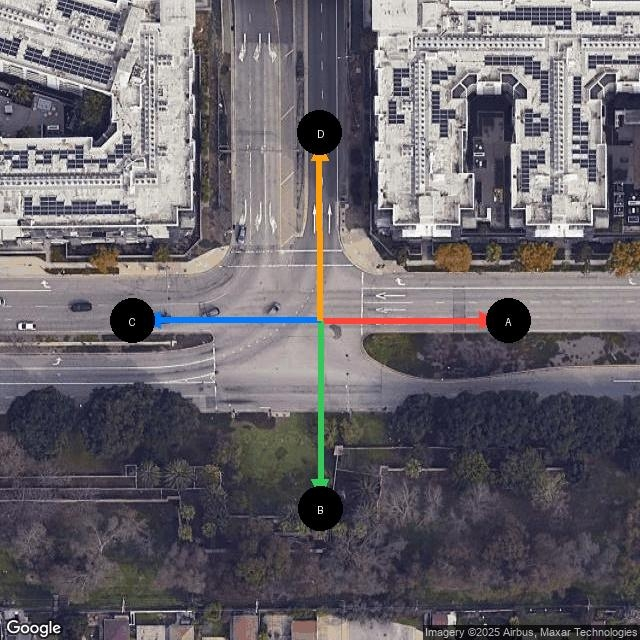
\includegraphics[width=\linewidth]{figures/failure-mode-3-map.jpg}
    \end{minipage}
    \hfill
    \begin{minipage}[t]{0.24\linewidth}
      \centering
      \vspace{0pt}
      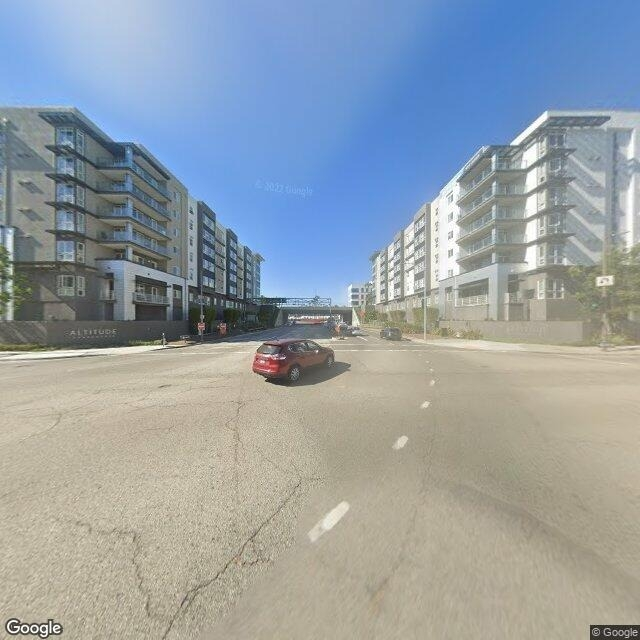
\includegraphics[width=\linewidth]{figures/failure-mode-3-sv.jpg}
    \end{minipage}
    \hfill
    \begin{minipage}[t]{0.50\linewidth}
      \vspace{0pt}
      \fbox{
        \begin{minipage}[t]{\linewidth}
        \footnotesize
        \textbf{Ground truth:} D, \textbf{Prediction:} A
        \medskip

        \textbf{Model trace (excerpt):}

        Direction A provides the most complete match. It correctly places large buildings on both sides of the road and crucially includes the distant underpass/bridge structure that is clearly visible in the street view photo.

        \medskip
        \textbf{Failure:}
        The model invents or misattributes a nonexistent large-scale structure (underpass/bridge) and then reasons as if it were present in the map.
        \end{minipage}
      }
    \end{minipage}
  
    \vspace{0.4em}
    \centering
    {\small\textbf{(d) False landmark projection}}
  \end{minipage}

  \vspace{0.5em}
  
  \caption{
  \textbf{More qualitative failure modes on m2sv.}
  Each row shows the same map--street-view pair with a different erroneous reasoning
  pattern exhibited by the model. From left to right: overhead map with candidate
  directions, corresponding street-view image, and an excerpt from the model’s
  reasoning trace highlighting the incorrect assumption. All examples are correctly
  solved by human annotators.
  }
  \label{fig:failure-examples-appendix}
  \end{figure*}